\begin{figure*}[b] %
  \centering
  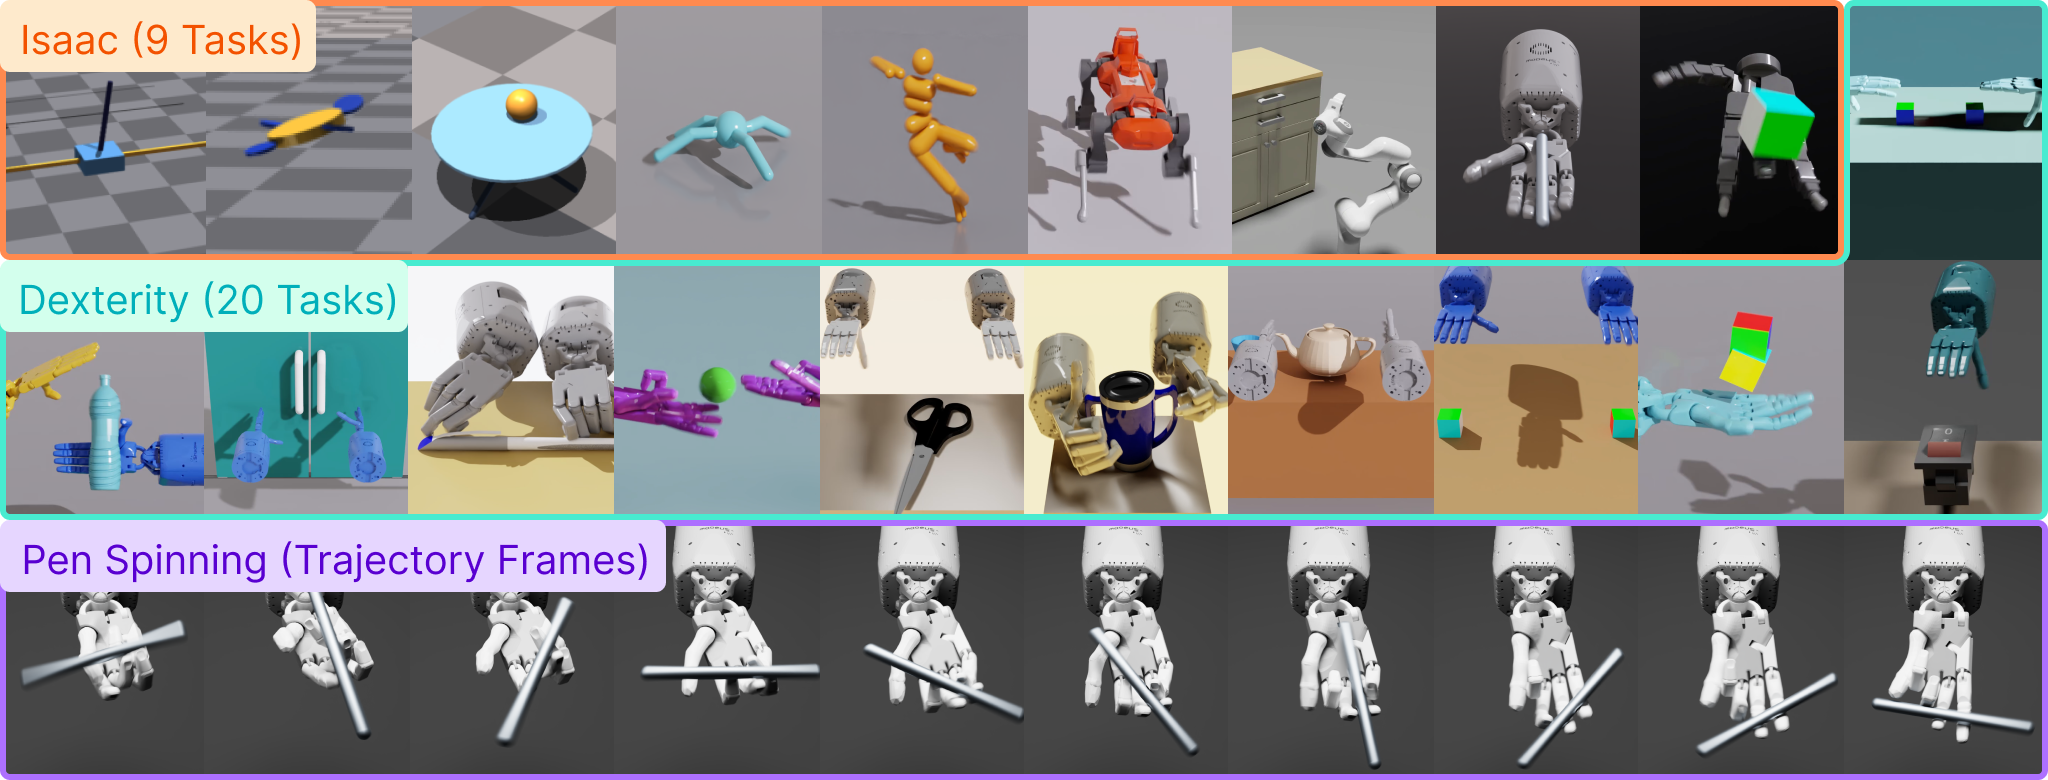
\includegraphics[width=0.9\textwidth]{figures/envs.png} %
  \caption{\ourmethod generates human-level reward functions across diverse robots and tasks. Combined with curriculum learning, \ourmethod for the first time, unlocks rapid pen-spinning capabilities on an anthropomorphic five-finger hand.}
  \label{fig:eureka}
\end{figure*}

\section{Introduction}

Large Language Models (LLMs) have excelled as high-level semantic planners for robotics tasks~\citep{ahn2022can, singh2023progprompt}, but whether they can be used to learn complex low-level manipulation tasks, such as dexterous pen spinning, remains an open problem. Existing attempts require substantial domain expertise to construct task prompts or learn only simple skills, leaving a substantial gap in achieving human-level dexterity~\citep{yu2023language, brohan2023rt}. 

On the other hand, reinforcement learning (RL) has achieved impressive results in dexterity~\citep{andrychowicz2020learning, handa2023dextreme} as well as many other domains-if the human designers can carefully construct reward functions that accurately codify and provide learning signals for the desired behavior; likewise, many real-world RL tasks admit sparse rewards that are difficult for learning, necessitating reward shaping that provides incremental learning signals. Despite their fundamental importance, reward functions are known to be notoriously difficult to design in practice~\citep{russell1995artificial, sutton2018reinforcement}; a recent survey conducted finds 92\% of polled reinforcement learning researchers and practitioners report manual trial-and-error reward design and 89\% indicate that their designed rewards are sub-optimal~\citep{booth2023perils} and lead to unintended behavior~\citep{hadfield2017inverse}.

Given the paramount importance of reward design, we ask whether it is possible to develop a \textit{universal} reward programming algorithm using state-of-the-art coding LLMs, such as GPT-4. Their remarkable abilities in code writing, zero-shot generation, and in-context learning have previously enabled effective programmatic agents~\citep{shinn2023reflexion, wang2023voyager}. Ideally, this reward design algorithm should achieve human-level reward generation capabilities that scale to a broad spectrum of tasks, including dexterity, automate the tedious trial-and-error procedure without human supervision, and yet be compatible with human oversight to assure safety and alignment.


\begin{figure*}[t!]
\centering 
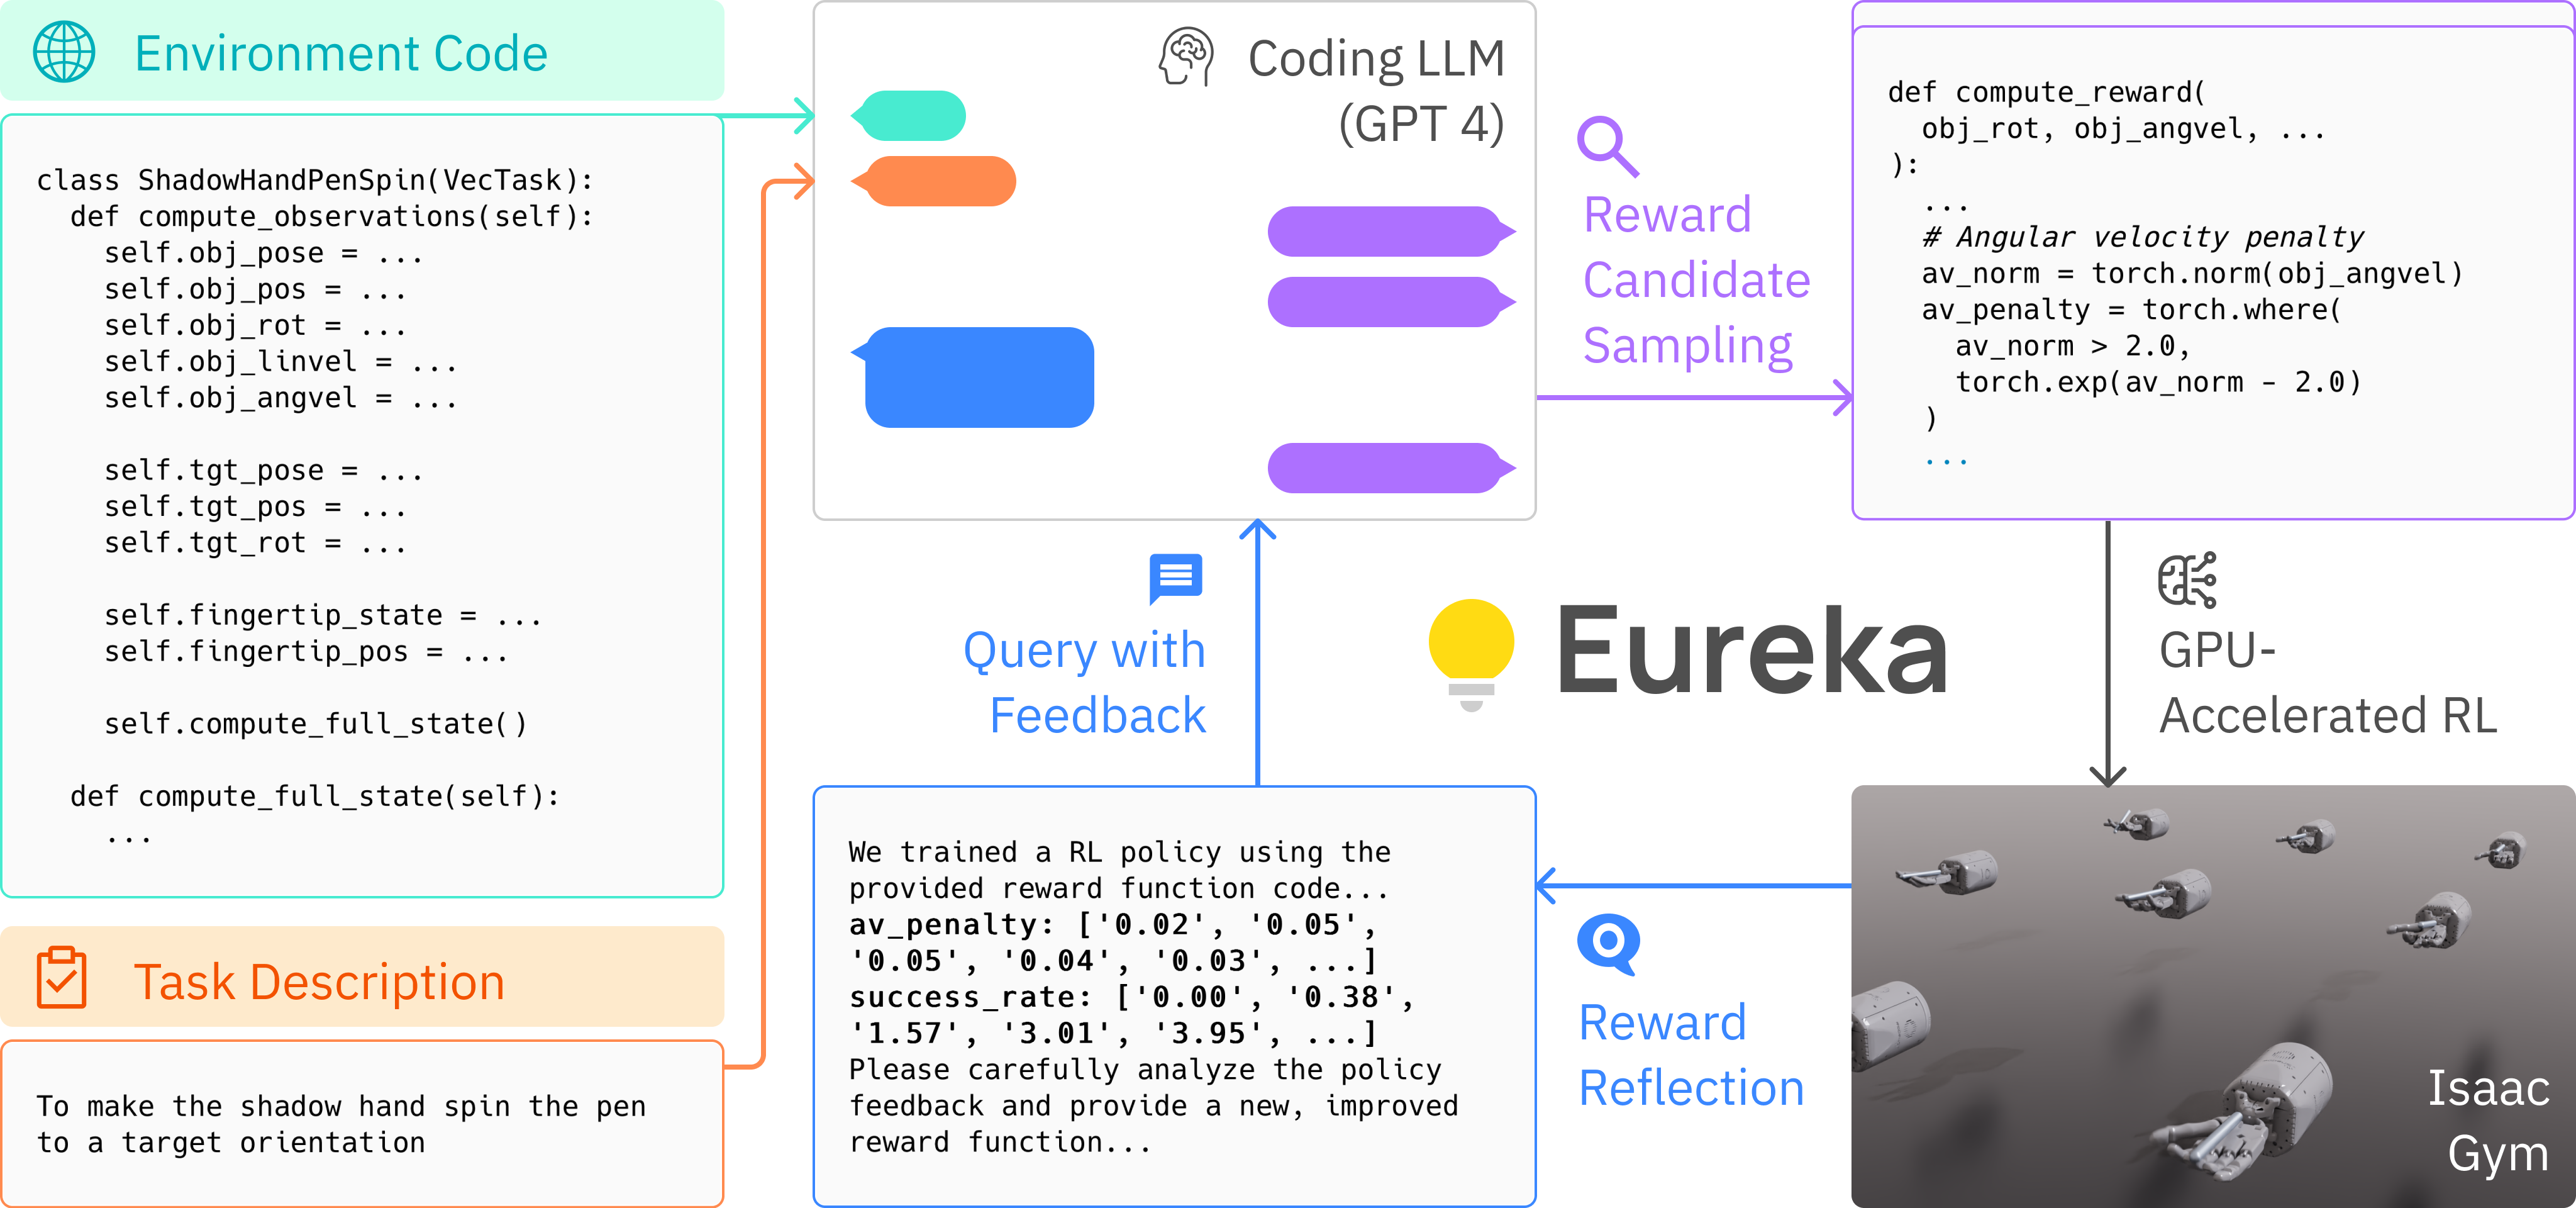
\includegraphics[width=\textwidth]{figures/eureka.png}
\caption{\ourmethod takes unmodified environment source code and language task description as context to zero-shot generate executable reward functions from a coding LLM. Then, it iterates between reward sampling, GPU-accelerated reward evaluation, and reward reflection to progressively improve its reward outputs.}
  \label{fig:eureka-concept}
\end{figure*}

We introduce \textbf{E}volution-driven \textbf{U}niversal \textbf{RE}ward \textbf{K}it for \textbf{A}gent (\ourmethod), a novel reward design algorithm powered by coding LLMs with the following contributions:
\begin{enumerate}[leftmargin=*]
\item \textbf{Achieves human-level performance on reward design} across a diverse suite of 29 open-sourced RL environments that include 10 distinct robot morphologies, including quadruped, quadcopter, biped, manipulator, as well as several dexterous hands; see Fig.~\ref{fig:eureka}. Without any task-specific prompting or reward templates, \ourmethod autonomously generates rewards that outperform expert human rewards on \textbf{83\%} of the tasks and realizes an average normalized improvement of \textbf{52\%}.

\item \textbf{Solves dexterous manipulation tasks that were previously not feasible by manual reward engineering}. We consider pen spinning, in which a five-finger hand needs to rapidly rotate a pen in pre-defined spinning configurations for as many cycles as possible. Combining \ourmethod with curriculum learning, we demonstrate for the first time rapid pen spinning maneuvers on a simulated anthropomorphic Shadow Hand (see Figure~\ref{fig:eureka} bottom). 

\item \textbf{Enables a new \textit{gradient-free} in-context learning approach to reinforcement learning from human feedback (RLHF)} that can generate more performant and human-aligned reward functions based on various forms of human inputs without model updating. We demonstrate that \ourmethod can readily benefit from and improve upon existing human reward functions. Likewise, we showcase \ourmethod's capability in using purely textual feedback to generate progressively more human-aligned reward functions. 


\end{enumerate}





  

Unlike prior work L2R on using LLMs to aid reward design~\citep{yu2023language}, \ourmethod is completely free of task-specific prompts, reward templates, as well as few-shot examples. In our experiments, \ourmethod significantly outperforms L2R due to its ability to generate free-form, expressive reward programs. \ourmethod's generality is made possible through three key algorithmic design choices: environment as context, evolutionary search, and reward reflection. First, by taking the \textbf{environment source code as context}, \ourmethod can zero-shot generate executable reward functions from the backbone coding LLM (GPT-4). Then, \ourmethod substantially improves the quality of its rewards by performing \textbf{evolutionary search}, iteratively proposing batches of reward candidates and refining the most promising ones within the LLM context window. This in-context improvement is made effective via \textbf{reward reflection}, a textual summary of the reward quality based on policy training statistics that enables automated and targeted reward editing; see Fig.~\ref{fig:eureka-reward} for an example of \ourmethod zero-shot reward as well as various improvements accumulated during its optimization. To ensure that \ourmethod can scale up its reward search to maximum potential, \ourmethod evaluates intermediate rewards using GPU-accelerated distributed reinforcement learning on IsaacGym~\citep{makoviychuk2021isaac}, which offers up to three orders of magnitude in policy learning speed, making \ourmethod an extensive algorithm that scales naturally with more compute. See Fig.~\ref{fig:eureka-concept} for an overview. We are committed to open-sourcing all prompts, environments, and generated reward functions to promote further research on LLM-based reward design.





























